\documentclass[a4paper]{article}
\usepackage[italian]{babel}
\usepackage[left=1cm, right=1cm, bottom=2cm, top=2cm]{geometry}
\usepackage{csvsimple}
\usepackage[utf8]{inputenc}
\usepackage{float}
\usepackage[table,xcdraw]{xcolor}
\usepackage[scaled]{helvet}
\renewcommand\familydefault{\sfdefault} 
\usepackage{pgfplots}
\pgfplotsset{compat=newest}
\usepackage{multicol}
\usepackage{tabularx}
\usepackage{xcolor}
%opening
\title{Relazione laboratorio Algoritmi Avanzati}
\author{Magarotto Francesco\\Muraro Enrico\\Piva Giulio}

\begin{document}
\rowcolors{2}{gray!25}{white}
\begin{titlepage}
  \vspace*{5cm}
  \begin{center}
    \Large\bfseries
	Relazione di laboratorio
  \end{center}
  \begin{center}
  \large
  Corso di Algoritmi Avanzati\\
  Laurea Magistrale in Informatica\\A.A. 2019-2020
  \end{center}
  \vspace{4cm plus 1fill}
  \begin{flushleft}
  \large
    Magarotto Francesco\\Muraro Enrico\\Piva Giulio
  \end{flushleft}
\end{titlepage}
\newpage
\begin{figure}[H]
\centering
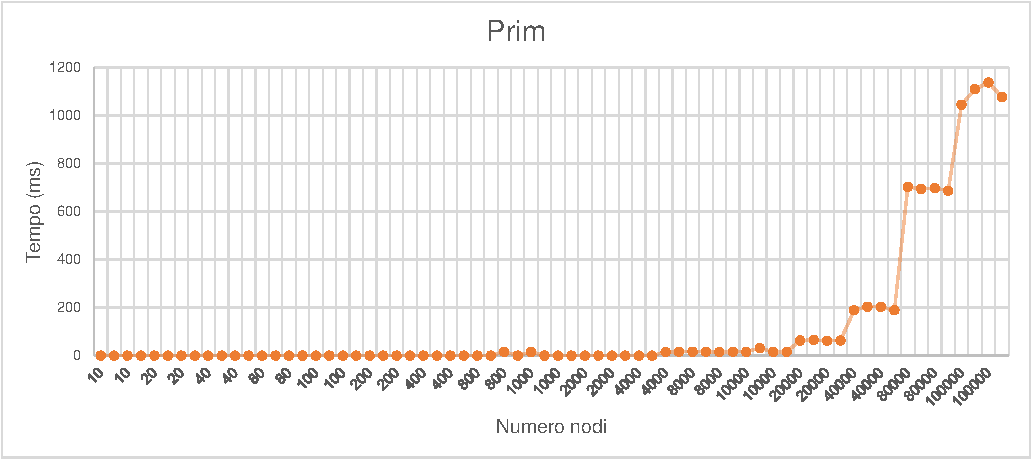
\includegraphics[scale=1]{grafici/prim.pdf}
\caption{Grafico andamento algoritmo di Prim}
\end{figure}

\begin{figure}[H]
\centering
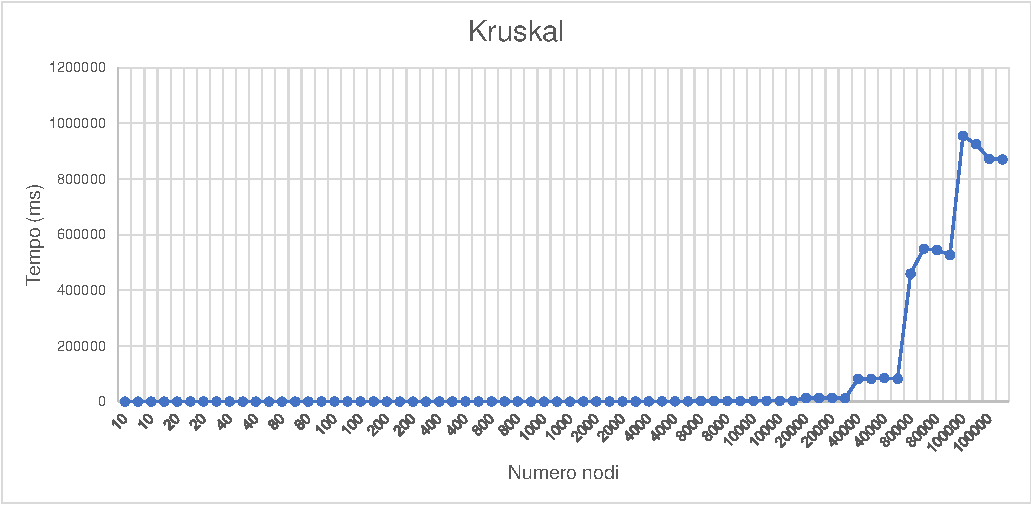
\includegraphics[scale=1]{grafici/kruskal.pdf}
\caption{Grafico andamento algoritmo di Kruskal}
\end{figure}

\begin{figure}[H]
\centering
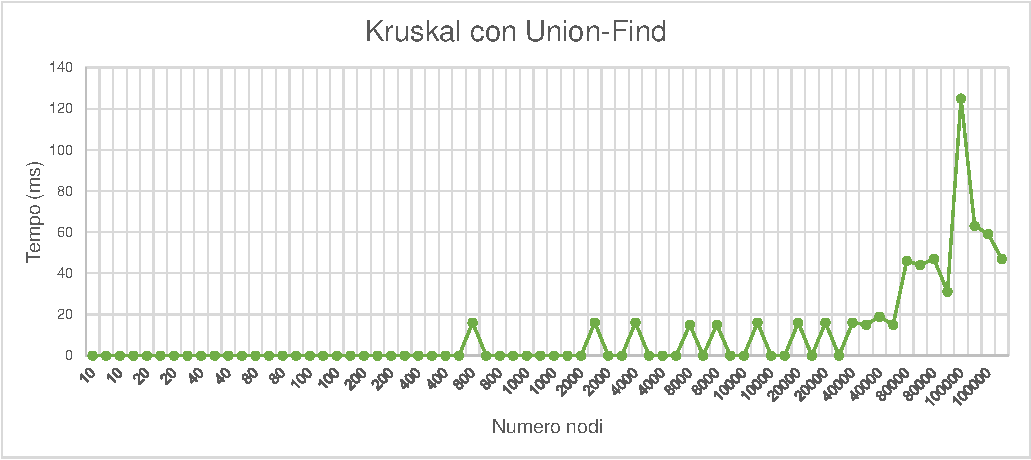
\includegraphics[scale=1]{grafici/kruskaluf.pdf}
\caption{Grafico andamento algoritmo di Kruskal con Union-Find}
\end{figure}

\begin{figure}[H]
\centering
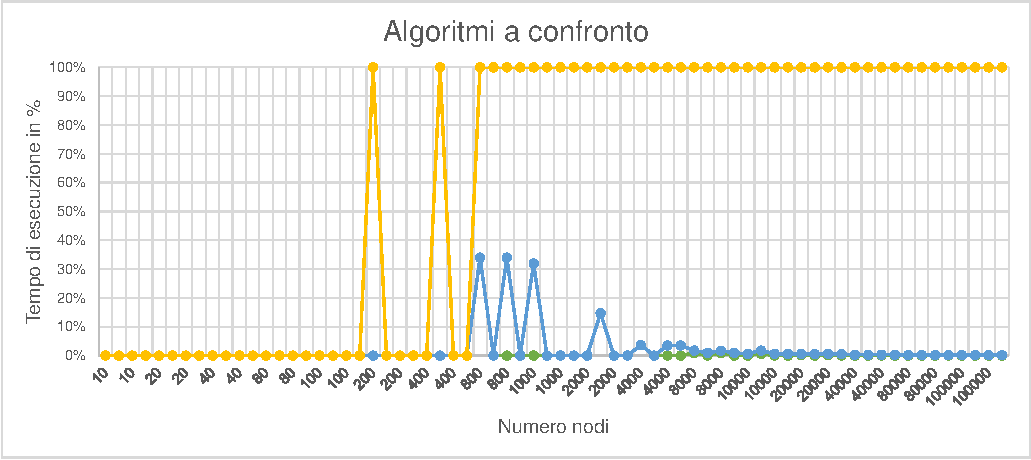
\includegraphics[scale=1]{grafici/confronto.pdf}
\caption{Grafico che mette in relazione i tempi di esecuzione dei tre algoritmi in base al tempo richiesto per la loro esecuzione}
\end{figure}

% Please add the following required packages to your document preamble:
% \usepackage[table,xcdraw]{xcolor}
% If you use beamer only pass "xcolor=table" option, i.e. \documentclass[xcolor=table]{beamer}
% Please add the following required packages to your document preamble:
% \usepackage[table,xcdraw]{xcolor}
% If you use beamer only pass "xcolor=table" option, i.e. \documentclass[xcolor=table]{beamer}
\begin{table}[]
\begin{minipage}[b]{10cm}
\begin{tabular}{|c|c|c|c|c|}
\rowcolor{gray!50}
\hline
\textbf{Nodi} & \textbf{Prim} & \textbf{Kruskal UF} & \textbf{Kruskal} & \textbf{MST} \\ \hline
10            & 0              & 0                   & 0                & 29316        \\ \hline
10            & 0              & 0                   & 0                & 2126         \\ \hline
10            & 0              & 0                   & 0                & -44765       \\ \hline
10            & 0              & 0                   & 0                & 20360        \\ \hline
20            & 0              & 0                   & 0                & -32021       \\ \hline
20            & 0              & 0                   & 0                & 18596        \\ \hline
20            & 0              & 0                   & 0                & -42560       \\ \hline
20            & 0              & 0                   & 0                & -37205       \\ \hline
40            & 0              & 0                   & 0                & -122078      \\ \hline
40            & 0              & 0                   & 0                & -37021       \\ \hline
40            & 0              & 0                   & 0                & -79570       \\ \hline
40            & 0              & 0                   & 0                & -79741       \\ \hline
80            & 0              & 0                   & 0                & -139926      \\ \hline
80            & 0              & 0                   & 0                & -211345      \\ \hline
80            & 0              & 0                   & 0                & -110571      \\ \hline
80            & 0              & 0                   & 0                & -233320      \\ \hline
100           & 0              & 0                   & 0                & -141960      \\ \hline
100           & 0              & 0                   & 0                & -271743      \\ \hline
100           & 0              & 0                   & 0                & -288906      \\ \hline
100           & 0              & 0                   & 0                & -232178      \\ \hline
200           & 0              & 0                   & 16               & -510185      \\ \hline
200           & 0              & 0                   & 0                & -515136      \\ \hline
200           & 0              & 0                   & 0                & -444357      \\ \hline
200           & 0              & 0                   & 0                & -393278      \\ \hline
400           & 0              & 0                   & 0                & -1122919     \\ \hline
400           & 0              & 0                   & 31               & -788168      \\ \hline
400           & 0              & 0                   & 0                & -895704      \\ \hline
400           & 0              & 0                   & 0                & -733645      \\ \hline
800           & 0              & 16                  & 31               & -1541291     \\ \hline
800           & 0              & 0                   & 32               & -1578294     \\ \hline
800           & 16             & 0                   & 31               & -1675534     \\ \hline
800           & 0              & 0                   & 15               & -1652119     \\ \hline
1000          & 15             & 0                   & 32               & -2091110     \\ \hline
1000          & 0              & 0                   & 32               & -1934208     \\ \hline
1000          & 0              & 0                   & 31               & -2229428     \\ \hline
1000          & 0              & 0                   & 31               & -2359192     \\ \hline
\end{tabular}
\end{minipage}
\begin{minipage}[b]{10cm}
\begin{tabular}{|c|c|c|c|c|}
\hline
\rowcolor{gray!50}
\textbf{Nodi} & \textbf{Prim} & \textbf{Kruskal UF} & \textbf{Kruskal} & \textbf{MST} \\ \hline
2000          & 0              & 0                   & 109              & -4811598     \\ \hline
2000          & 0              & 16                  & 93               & -4739387     \\ \hline
2000          & 0              & 0                   & 109              & -4717250     \\ \hline
2000          & 0              & 0                   & 125              & -4537267     \\ \hline
4000          & 0              & 16                  & 423              & -8722212     \\ \hline
4000          & 0              & 0                   & 437              & -9314968     \\ \hline
4000          & 15             & 0                   & 412              & -9845767     \\ \hline
4000          & 16             & 0                   & 439              & -8681447     \\ \hline
8000          & 16             & 15                  & 1722             & -17844628    \\ \hline
8000          & 16             & 0                   & 1713             & -18800966    \\ \hline
8000          & 15             & 15                  & 1731             & -18741474    \\ \hline
8000          & 16             & 0                   & 1753             & -18190442    \\ \hline
10000         & 16             & 0                   & 2637             & -22086729    \\ \hline
10000         & 31             & 16                  & 2601             & -22338561    \\ \hline
10000         & 15             & 0                   & 2563             & -22581384    \\ \hline
10000         & 16             & 0                   & 2638             & -22606313    \\ \hline
20000         & 63             & 16                  & 12976            & -45978687    \\ \hline
20000         & 65             & 0                   & 13002            & -45195405    \\ \hline
20000         & 62             & 16                  & 13009            & -47854708    \\ \hline
20000         & 63             & 0                   & 12427            & -46420311    \\ \hline
40000         & 189            & 16                  & 81522            & -92003321    \\ \hline
40000         & 203            & 15                  & 81525            & -94397064    \\ \hline
40000         & 203            & 19                  & 84400            & -88783643    \\ \hline
40000         & 189            & 15                  & 81242            & -93017025    \\ \hline
80000         & 703            & 46                  & 459713           & -186834082   \\ \hline
80000         & 694            & 44                  & 549392           & -185997521   \\ \hline
80000         & 697            & 47                  & 545050           & -182065015   \\ \hline
80000         & 687            & 31                  & 526711           & -180803872   \\ \hline
100000        & 1045           & 125                 & 955113           & -230698391   \\ \hline
100000        & 1110           & 63                  & 925063           & -230168572   \\ \hline
100000        & 1137           & 59                  & 872704           & -231393935   \\ \hline
100000        & 1077           & 47                  & 869876           & -231011693   \\ \hline
\end{tabular}
\end{minipage}
\caption{Tabella dei risultati. Per ogni algoritmo, i valori si riferiscono al tempo di esecuzione, espressi in ms, di quell'algoritmo con un grafo avente $n$ nodi.}
\end{table}
\end{document}
